%!TEX root = Thesis_main.tex
\chapter*{Appendices}
\clearpage
\addcontentsline{toc}{chapter}{Appendices}
\section{Super Mega Bot Datasheet}
\label{AppA}

\begin{figure}[h]
	\begin{center} 
		\subfigure[Supermegabot]{
		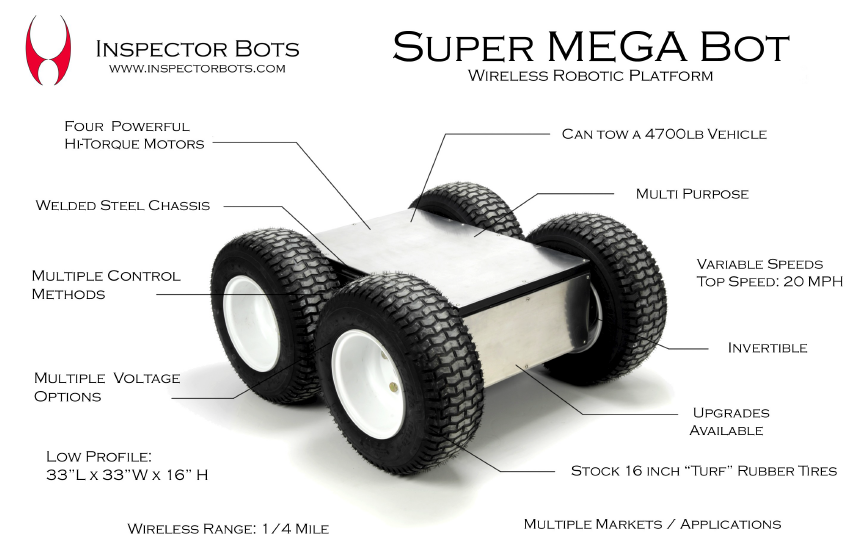
\includegraphics[scale=0.43]{SuperMegaBot}
		\centering
		\label{fig:SuperMegaBot}}
		\qquad
		\subfigure[Wiring scheme]{
		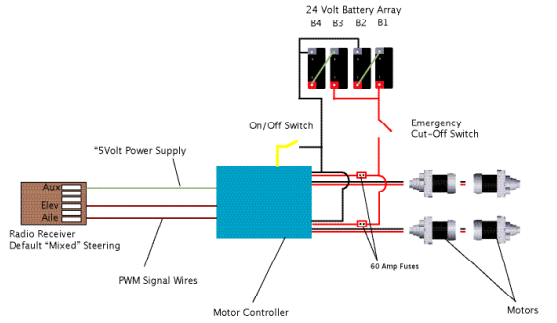
\includegraphics[scale=0.43]{SMBwires}
		\centering
		\label{SMB Wiring}}
	\end{center}
\end{figure}

Its base model comes with:\\
•	Chassis: Powder Coated Steel and Aluminum \\
•	Dimensions: 84cm L x 84cm W x 40.64cm H, Weight: 109 kg\\
•	Drive: Four Electric Motors\\
•	Load Capacity: 113,5 kg\\
•	Speed Controllers: RoboteQ 2x VDC2450\\
•	Speed: 0-16 km/h \\
•	Suspension: Rigid\\
•	Tires: Interchangeable, Pneumatic, 40.64cm Diameter Turf Tires\\
\url{https://www.youtube.com/watch?v=3X8IWnR1QDI}

%%%%%%%%%%%%%%%%%%%%%%%%%%%%%%%%%%%%%%%%%%%%%%%%%%%%%%%%%%%%%%%%%%%%%%%%%%%%%%%%%%%%%%%%%%%%%%%%%%%%%%%%%%%%%%%%%%%%%%



% \begin{figure}[!th]
% 	\begin{center} 
% 		\centerline{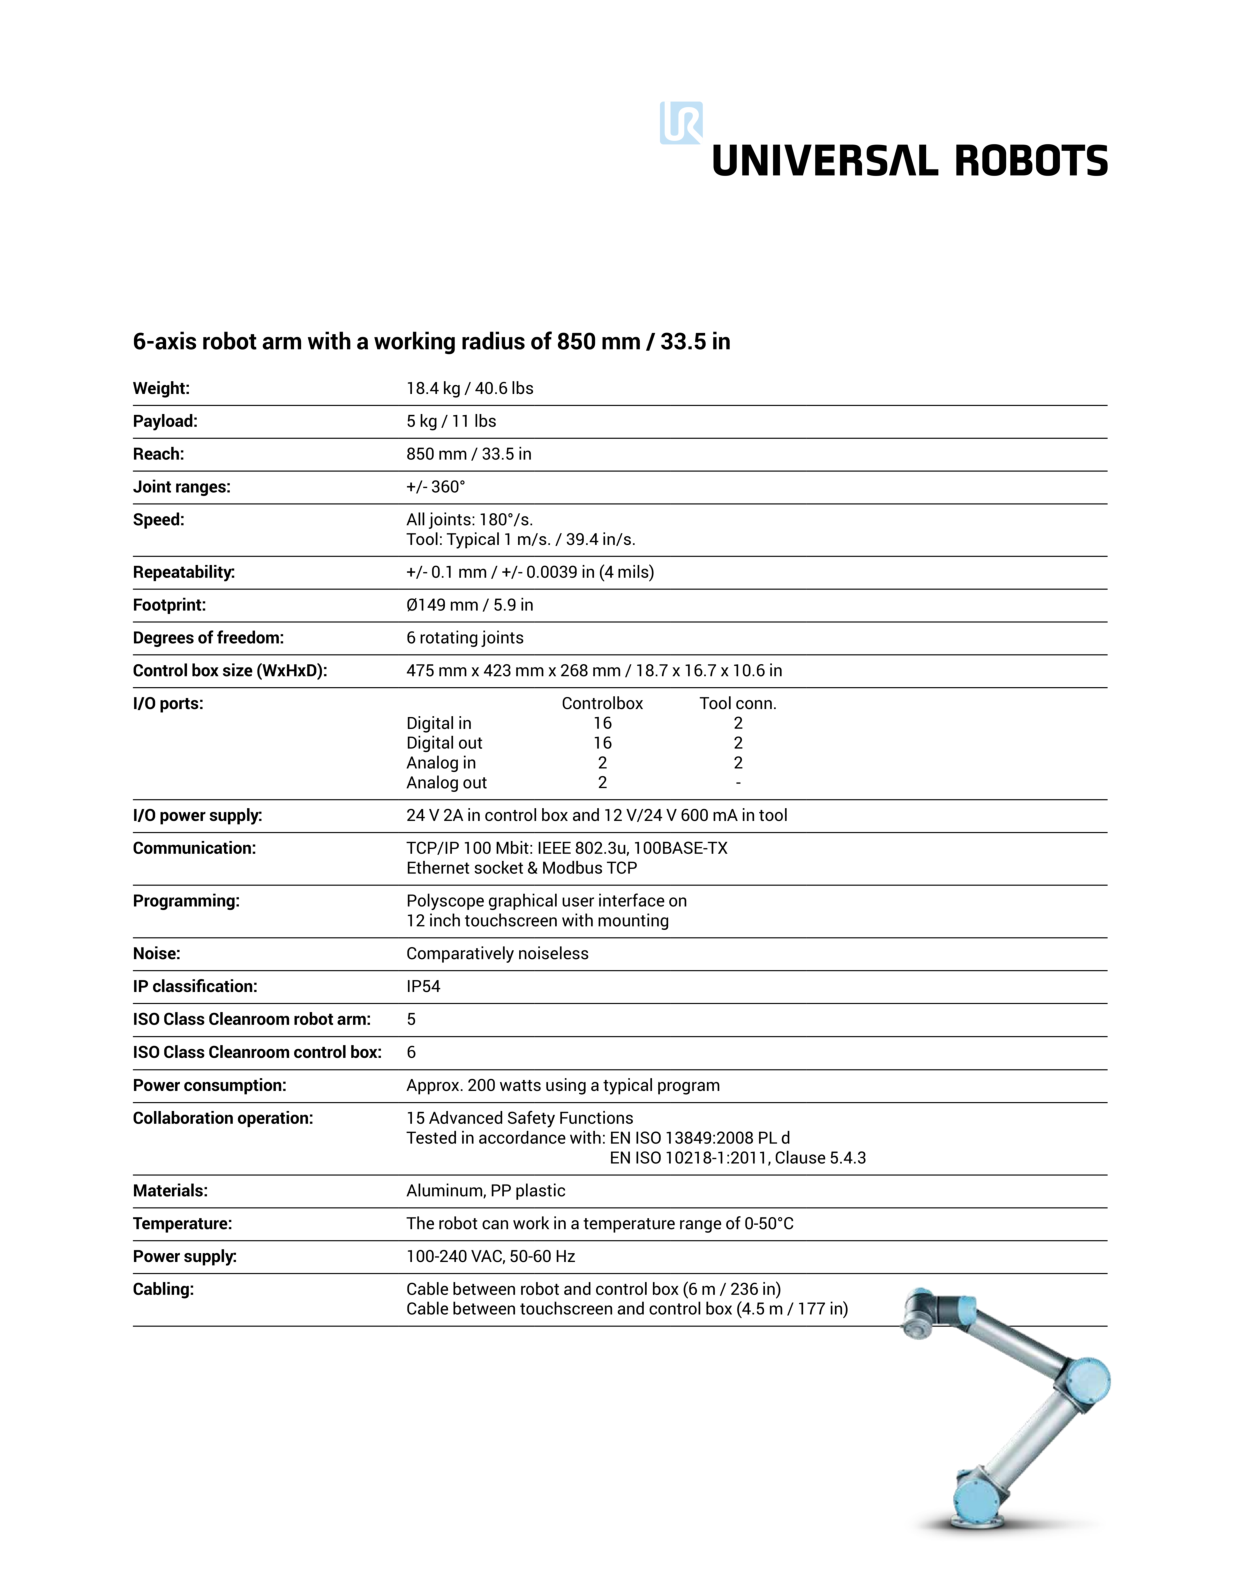
\includegraphics[scale=0.9]{ur5_en_V2}}
% 		\label{SMB Wiring} 
% 	\end{center}
% \end{figure}
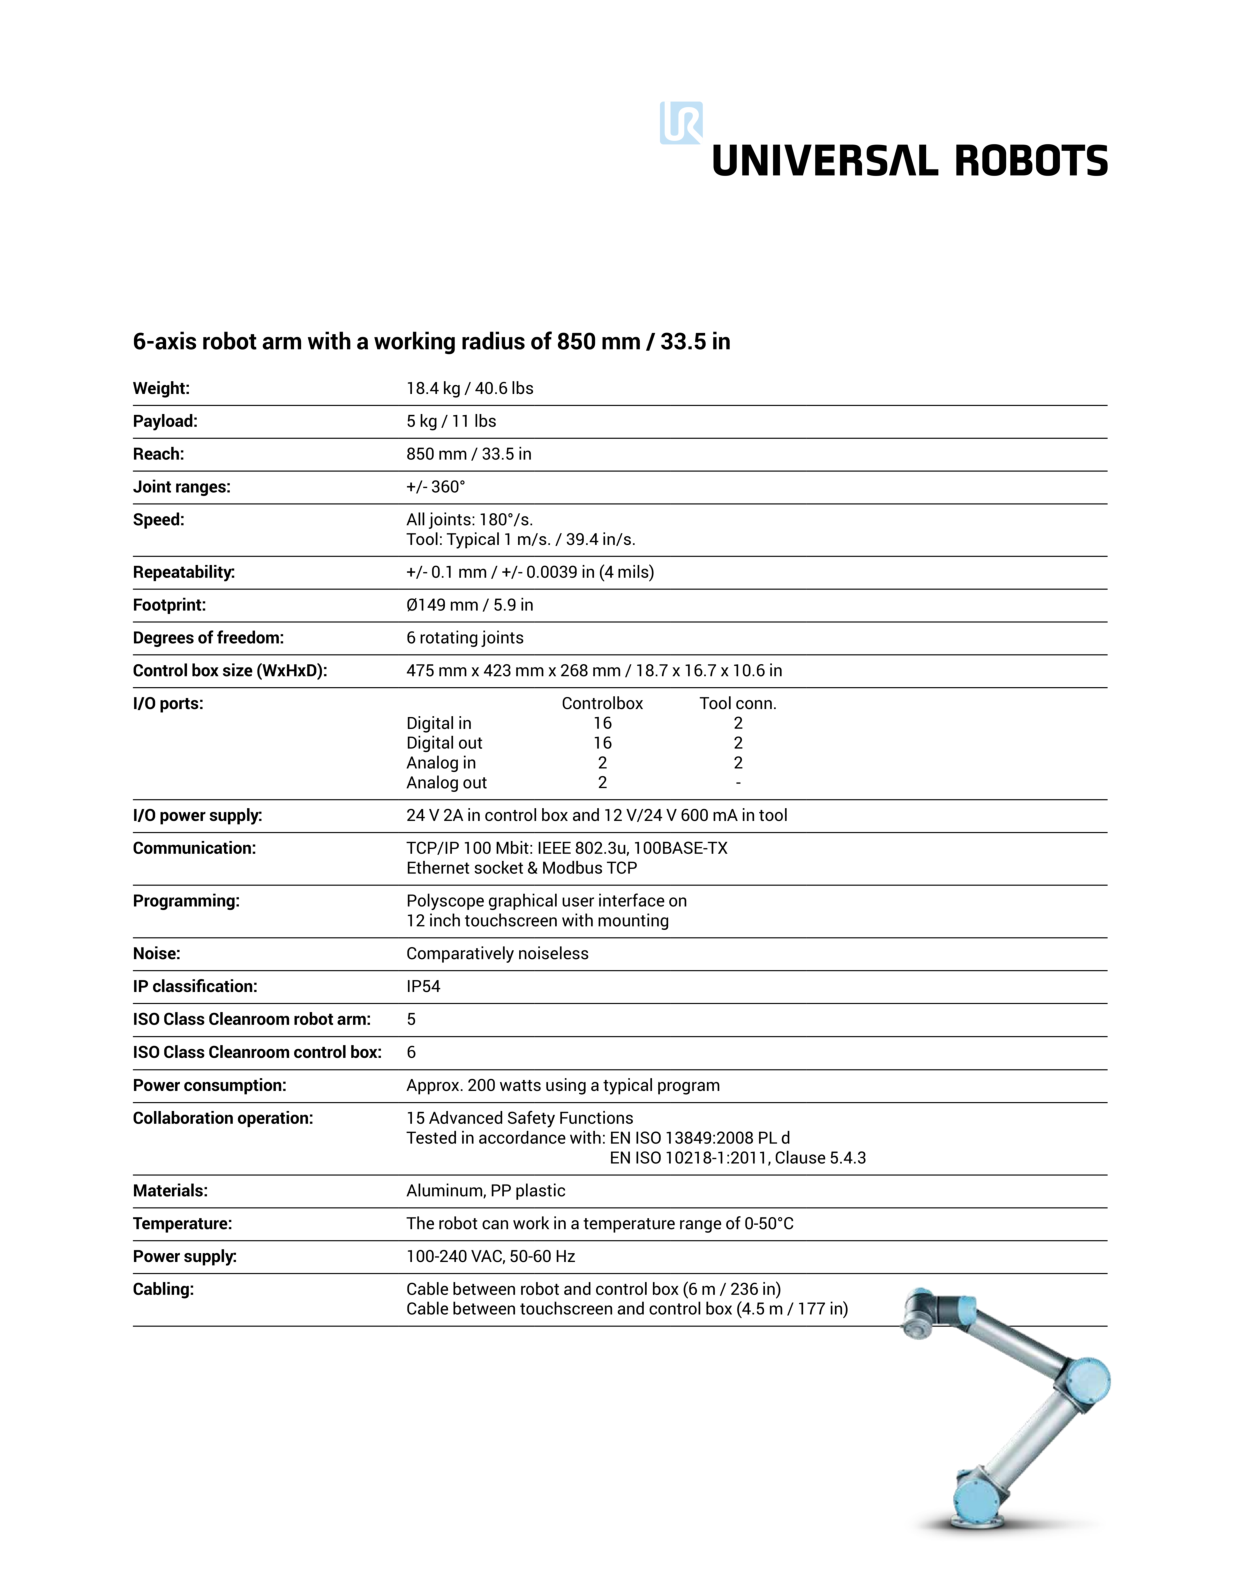
\includepdf[pagecommand={\section{UR5 Datasheet}}, offset=15 0]{ur5_en_V2.pdf}
\label{AppB}

%%%%%%%%%%%%%%%%%%%%%%%%%%%%%%%%%%%%%%%%%%%%%%%%%%%%%%%%%%%%%%%%%%%%%%%%%%%%%%%%%%%%%%%%%%%%%%%%%%%%%%%%%%%%%%%%%%%%%%

\section{Interior Point OPTimizer (IPOPT)}
\label{AppC}



IPOPT (\underline{I}nterior \underline{P}oint \underline{Opt}imizer,
pronounced ``Eye--Pea--Opt'') is an open source software package for
large-scale nonlinear optimization. It can be used to solve general
nonlinear programming problems of the form
%\begin{subequations}\label{NLP}
\begin{eqnarray*}
\min_{x\in\RR^n} &&f(x) \label{eq:obj} \\
\mbox{s.t.} \;  &&g^L \leq g(x) \leq g^U \label{eq:constraints}\\
                &&x^L \leq x \leq x^U, \label{eq:bounds}
\end{eqnarray*}
%\end{subequations}
where $x \in \RR^n$ are the optimization variables (possibly with
lower and upper bounds, $x^L\in(\RR\cup\{-\infty\})^n$ and
$x^U\in(\RR\cup\{+\infty\})^n$), $f:\RR^n\longrightarrow\RR$ is the
objective function, and $g:\RR^n\longrightarrow \RR^m$ are the general
nonlinear constraints.  The functions $f(x)$ and $g(x)$ can be linear
or nonlinear and convex or non-convex (but should be twice
continuously differentiable). The constraints, $g(x)$, have lower and
upper bounds, $g^L\in(\RR\cup\{-\infty\})^m$ and
$g^U\in(\RR\cup\{+\infty\})^m$. Note that equality constraints of the
form $g_i(x)=\bar g_i$ can be specified by setting
$g^L_{i}=g^U_{i}=\bar g_i$. \\

More information aboit Interior point method can be found in \cite{polik2010interior}.
IPOPT technical informations can be found at \url{https://projects.coin-or.org/Ipopt}.

% In the following table the specifications given by Universal Robots are stated. 
% \begin{table}
% 	\begin{tabular}{p{4cm} | p{3cm} p{3cm}}
% 		\hline
% 		Performance & \multicolumn{2}{l}{ } \\
% 		\hline \hline
% 		Repeatibility & \multicolumn{2}{l}{$\pm$ 0.1 mm} \\
% 		Ambient temperature range & \multicolumn{2}{l}{0-50°} \\
% 		Power Consumption  & \multicolumn{2}{l}{Min 90W, Typical 150W, Max 325W} \\
% 		Collaboration operation & \multicolumn{2}{l}{15 advanced adjustable safety functions} \\
% 		\hline \hline
% 		Specifications & \multicolumn{2}{l}{ }\\
% 		\hline \hline 
% 		Payload & \multicolumn{2}{l}{5 kg} \\
% 		Reach & \multicolumn{2}{l}{850 mm} \\
% 		Degrees of freedom & \multicolumn{2}{l}{6 rotating joints} \\
% 		Programming & \multicolumn{2}{l}{Polyscope graphical user interface on 12 inch touchscreen} \\
% 		\hline \hline
% 		Movement & & \\
% 		\hline 
% 		& Working range & Maximum speed \\
% 		\hline \hline
% 		Base & $\pm$ 360°  & $\pm$ 180°/sec \\
% 		Shoulder & $\pm$ 360° & $\pm$ 180°/sec \\
% 		Wrist1 & $\pm$ 360° & $\pm$ 180°/sec \\
% 		Wrist2 & $\pm$ 360° & $\pm$ 180°/sec \\
% 		Wrist3 & $\pm$ 360° & $\pm$ 180°/sec \\
% 		Typical tool & & 1m/sec \\
% 		\hline \hline
% 		Physical & \multicolumn{2}{l}{ }\\
% 		\hline \hline
% 		Footprint & \multicolumn{2}{l}{\o 149mm} \\
% 		Materials & \multicolumn{2}{l}{Aluminium, PP Plastics} \\
% 		Weight (with cable) & 18.4 kg 
% 	\end{tabular}
% \end{table}